\section{Presentation Logic Layer}

%What pages will be present in your project? briefly indicate how your web site will be organized

The website is divided into the following pages:
\begin{itemize}
    \item Homepage: contains the showcase of the featured products and the available products.
    \item Product page: allows the customer to inspect all the information about the given product. To buy the product the customer has to be logged in.
    \item Login page: allows both customers and employees to login. 
    \item Order list and Order details page: allow each customer to look at their order history to open a ticket, cancel the order or get the invoice.
    \item Tickets page: allows each customer to look at their ticket history. There exists an employee version of the page to manage each ticket.
    \item Product management pages: both simple employees and administrators are able to look at all the products and edit/delete them. Through a second page (Discount management) it is also possible to add some discounts.
    \item Orders management page: both simple employees and administrators are able to look at all the orders and edit/cancel them. It's also possible to look at the existing invoices for each product.
    \item User edit page: allows both customers and employees to modify their personal data using a simple form. 
    \item Administration page: allows the administrators to edit the name, surname, role of all the users and even delete their account.
\end{itemize}

\subsection{Homepage}
    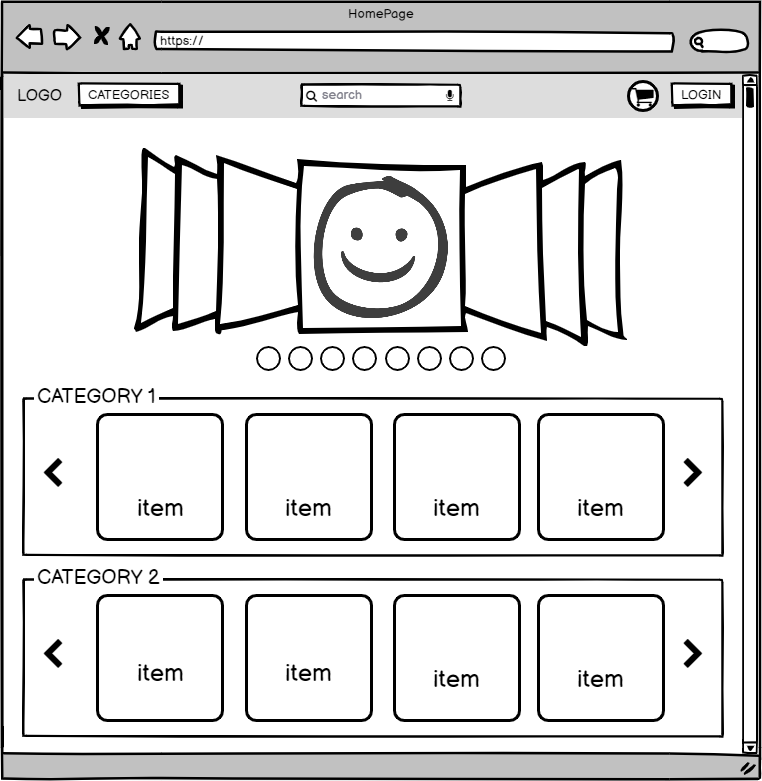
\includegraphics[width=\textwidth,height=\textheight,keepaspectratio]{mockups/homepageMockup.png}
\\
The homepage contains the main information regarding the various products available.
The products are divided into subsets according to their category.This subdivision will be done by means of a scrollable list. Moreover, the homepage contains a bar to search by name of the single elements.
Like most of the top pages, the homepage contains a status bar that allows the user to register, log in or log out once logged in.
Finally, this status bar allows customers to show the history of the products purchased.

\subsection{Product page}
    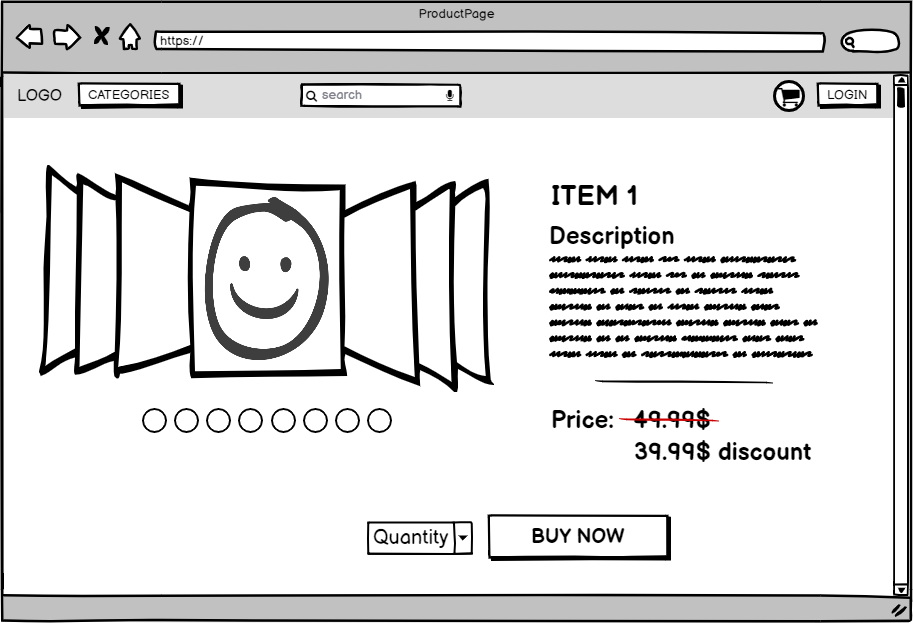
\includegraphics[width=\textwidth,height=\textheight,keepaspectratio]{mockups/productPageMockup.png}
\\
The product page shows in detail the information regarding the individual product.
This page shows all the pictures available for a given product, the description and its price.
In addition, it also shows any discount applied to the product.
If the customer is logged in, it will be possible for him to purchase the product within the maximum quantity available. It is possible to enter these particular pages by clicking on the product on the homepage or by searching by product name.

\subsection{OrderList and OrderDetails}
    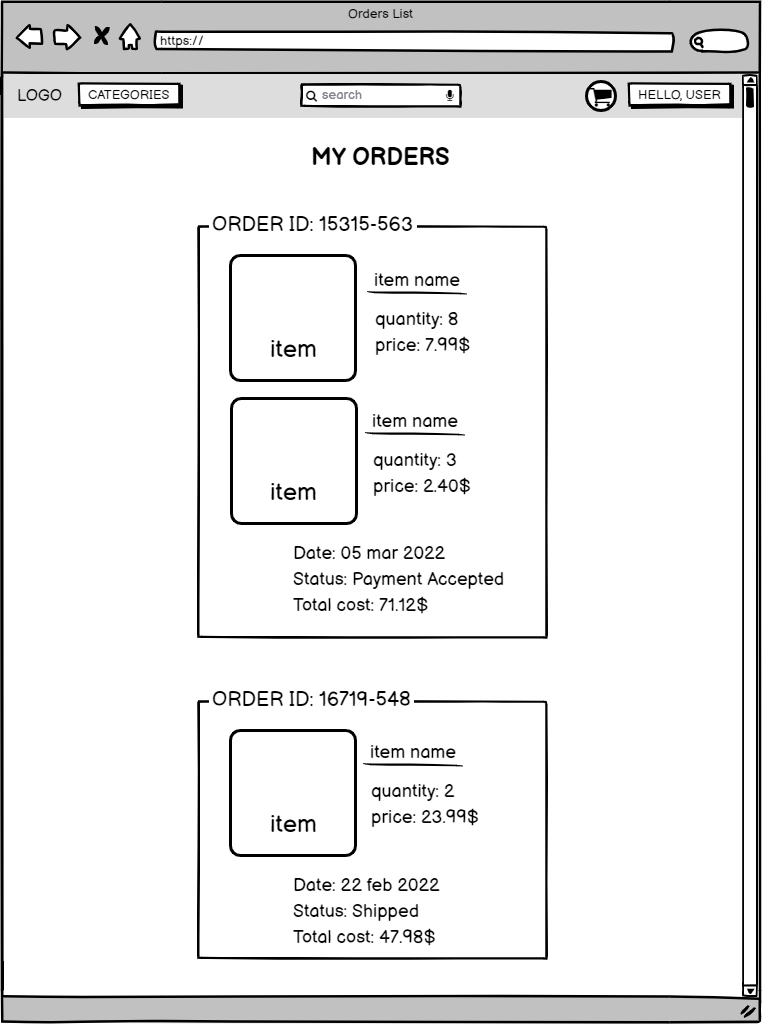
\includegraphics[width=\textwidth,height=\textheight,keepaspectratio]{mockups/ordersPageMockup.png}
\\
This page shows in detail all the orders placed by the given customer user, once logged in. It shows the history of all orders placed since the user's registration to the site. For each order it shows the date, the total price and the status of the order.
Furthermore, it shows the list of all the products purchased in the given order, the quantity of each and the unit price at the time of purchase.

\subsection{Ticket list management}
    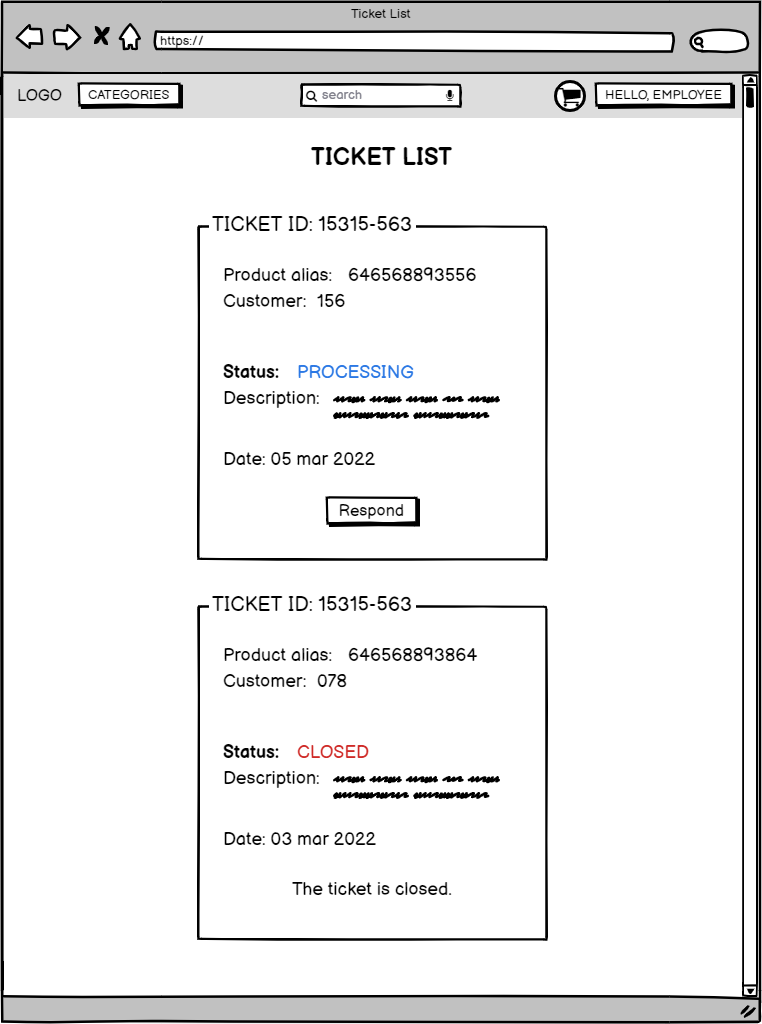
\includegraphics[width=\textwidth,height=\textheight,keepaspectratio]{mockups/ticketPageMockup.png}
\\
The ticket list page can be accessed by both customers and employees. In the customer version, the page shows the list of the ticket opened by the user. Each ticket displays its ID, its status and the product involved. In the employee version, each ticket shows also the ID of the customer. Furthermore, this page allows the employee to respond to the ticket and update its status.


\subsection{UserEdit page}
    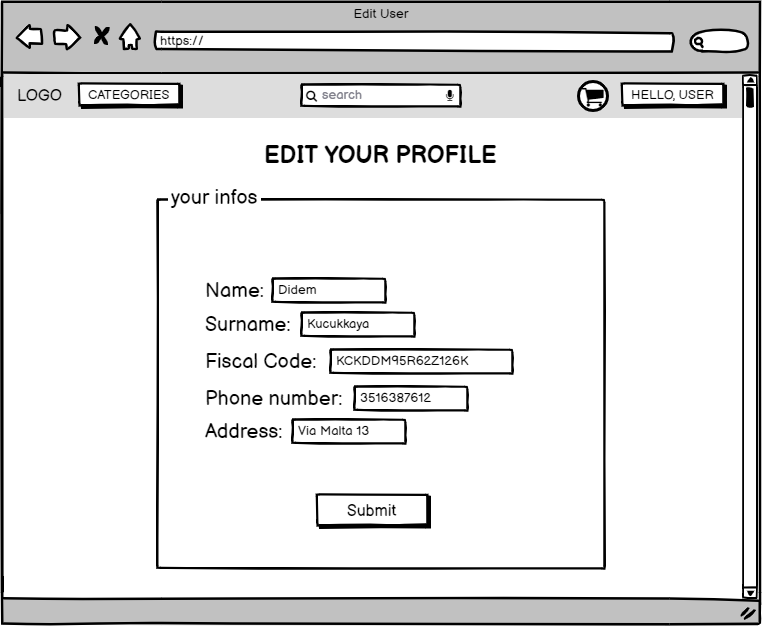
\includegraphics[width=\textwidth,height=\textheight,keepaspectratio]{mockups/userEditPageMockup.png}

The user edit page allows the customer type user to change their personal data.The page will consist of text boxes with default values corresponding to the values previously entered by the user. The page allows you to change data such as telephone number, name, surname but not unique / primary key data. This is because these particular data are used for login, and to avoid conflicts it was decided to do so.
Obviously this page will be available only after the user login.
    
\subsection{Admin: product management}
    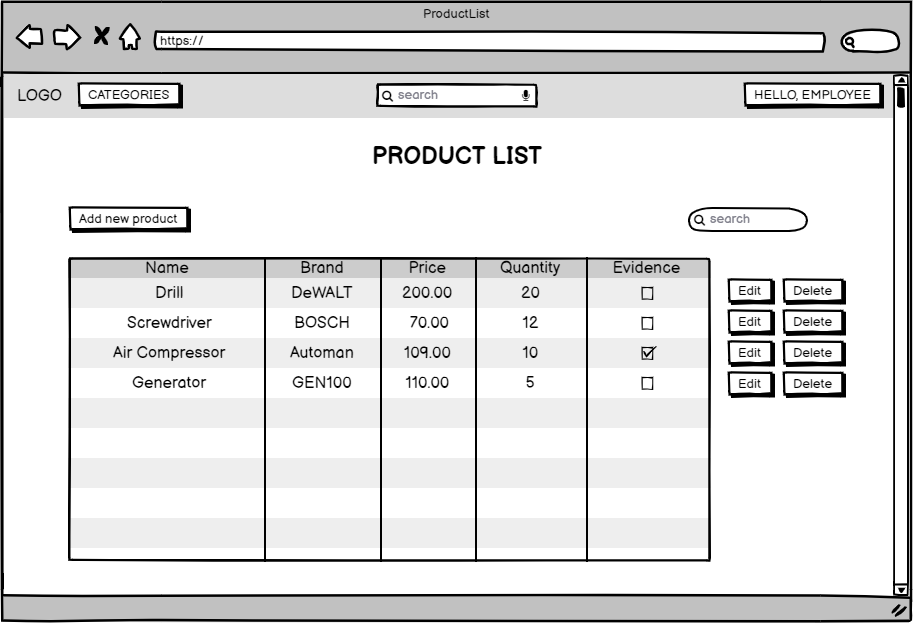
\includegraphics[width=\textwidth,height=\textheight,keepaspectratio]{mockups/productListPageMockup.png}
    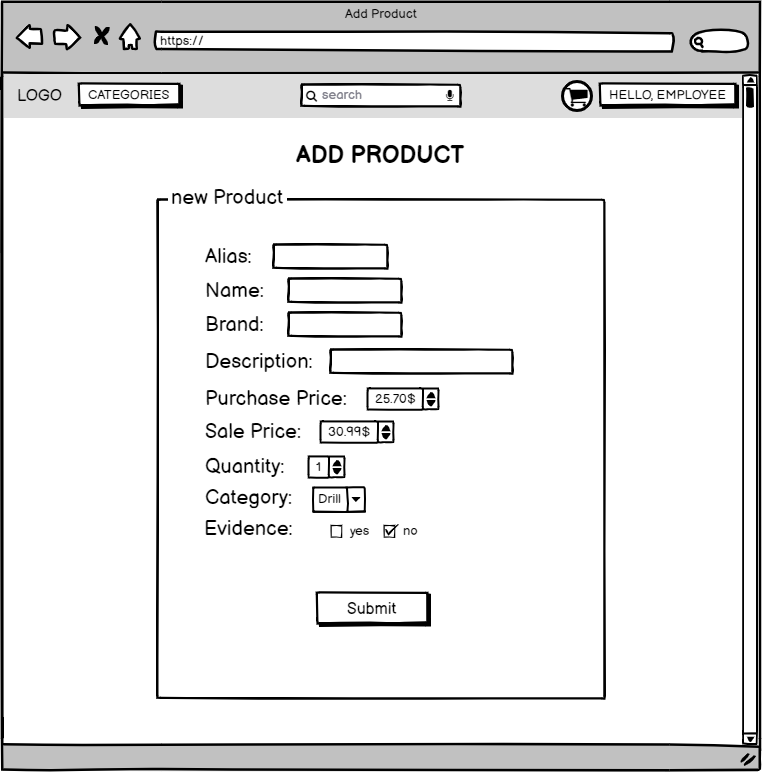
\includegraphics[width=\textwidth,height=\textheight,keepaspectratio]{mockups/addProductPageMockup.png}
\\
The product management pages can be accessed only by employees (and thus by administrators as well). The product list page displays and allows to edit and delete every product (even the ones with quantity equals to zero). It also allows to add a new product, through the add product page. Since every product belongs to a specific category, it is also possible to add a new category when adding a new product.  


\subsection{Admin: user management}
    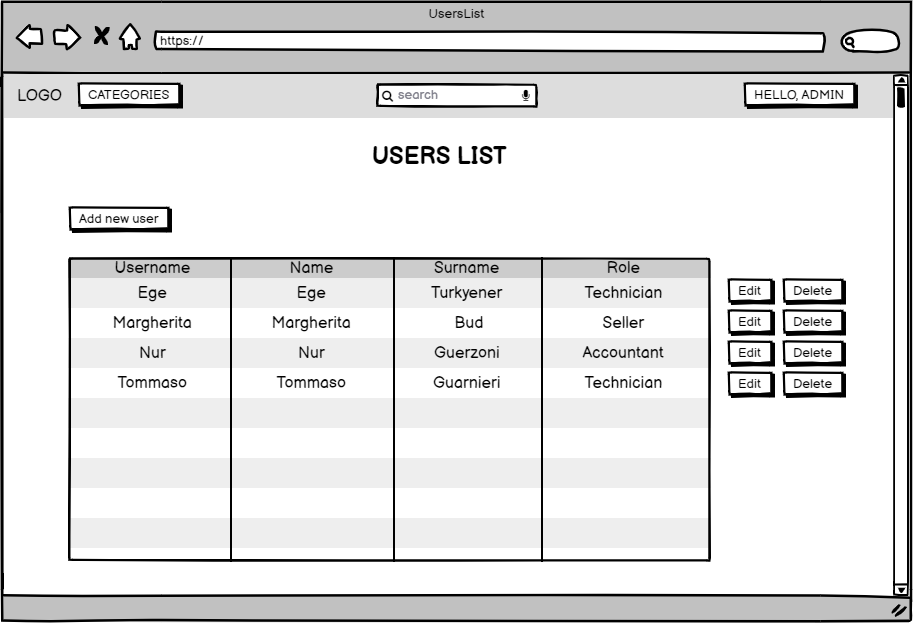
\includegraphics[width=\textwidth,height=\textheight,keepaspectratio]{mockups/usersListPageMockup.png}
\\
    The user management page can be reached only by administrators. The page displays the username, name, surname and role of any employee registered in the website. It is also possible to edit these informations, add a new employee and delete any employee account.

